
\subsection{Working with Sequences and their Formula}

\begin{defn}[Sequence]
    A \emph{sequence} is an ordered list of numbers or objects such as
    \[s_0=0, s_1=2, s_2=4, s_3=6, \ldots .\]
    In this sequence we say that \(s_0\) is the \emph{initial term}, each subscript is called an \emph{index}, and \(s_n=2n\) would be the \emph{explicit} or \emph{general} formula.
    \index{sequence}\index{index}\index{explicit formula}\index{general formula}
\end{defn}

% Decreasing
\begin{exposition}
Consider the sequence with explicit formula \(a_n=1/2^n\):
\begin{sides}
    \begin{itemize}
        \item \(a_0=1/2^0=1\)
        \item \(a_1=1/2^1=1/2\)
        \item \(a_2=1/2^2=1/4\)
        \item \(a_3=1/2^3=1/8\)
        \item \(a_4=1/2^4=1/16\)
        \item \(a_5=1/2^5=1/32\)
    \end{itemize}
    Description: Bounded and decreasing
    \index{bounded}\index{decreasing}
\tcblower
    % \inputtikz{filled_out_seq_graph}
    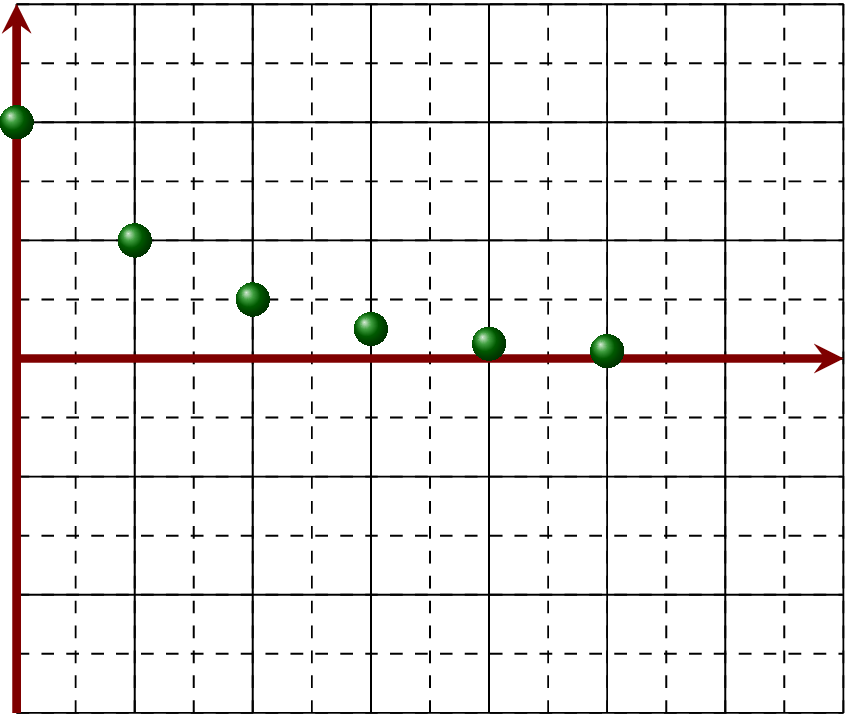
\includegraphics[scale=0.24,alt={Graph showing values in a sequence},width=0.75\linewidth]{images/created/filled_out_seq_graph.png}
\end{sides}
\end{exposition}

% \clearpage

% Increasing
\begin{practiceprob}
Consider the sequence \(b_n=2^n\):
\begin{sides}
    \begin{itemize}
        \item \(b_0=\)
        \item \(b_1=\)
        \item \(b_2=\)
        \item \(b_3=\)
        \item \(b_4=\)
    \end{itemize}
    Description:
\tcblower
    % \inputtikz{empty_seq_graph}
    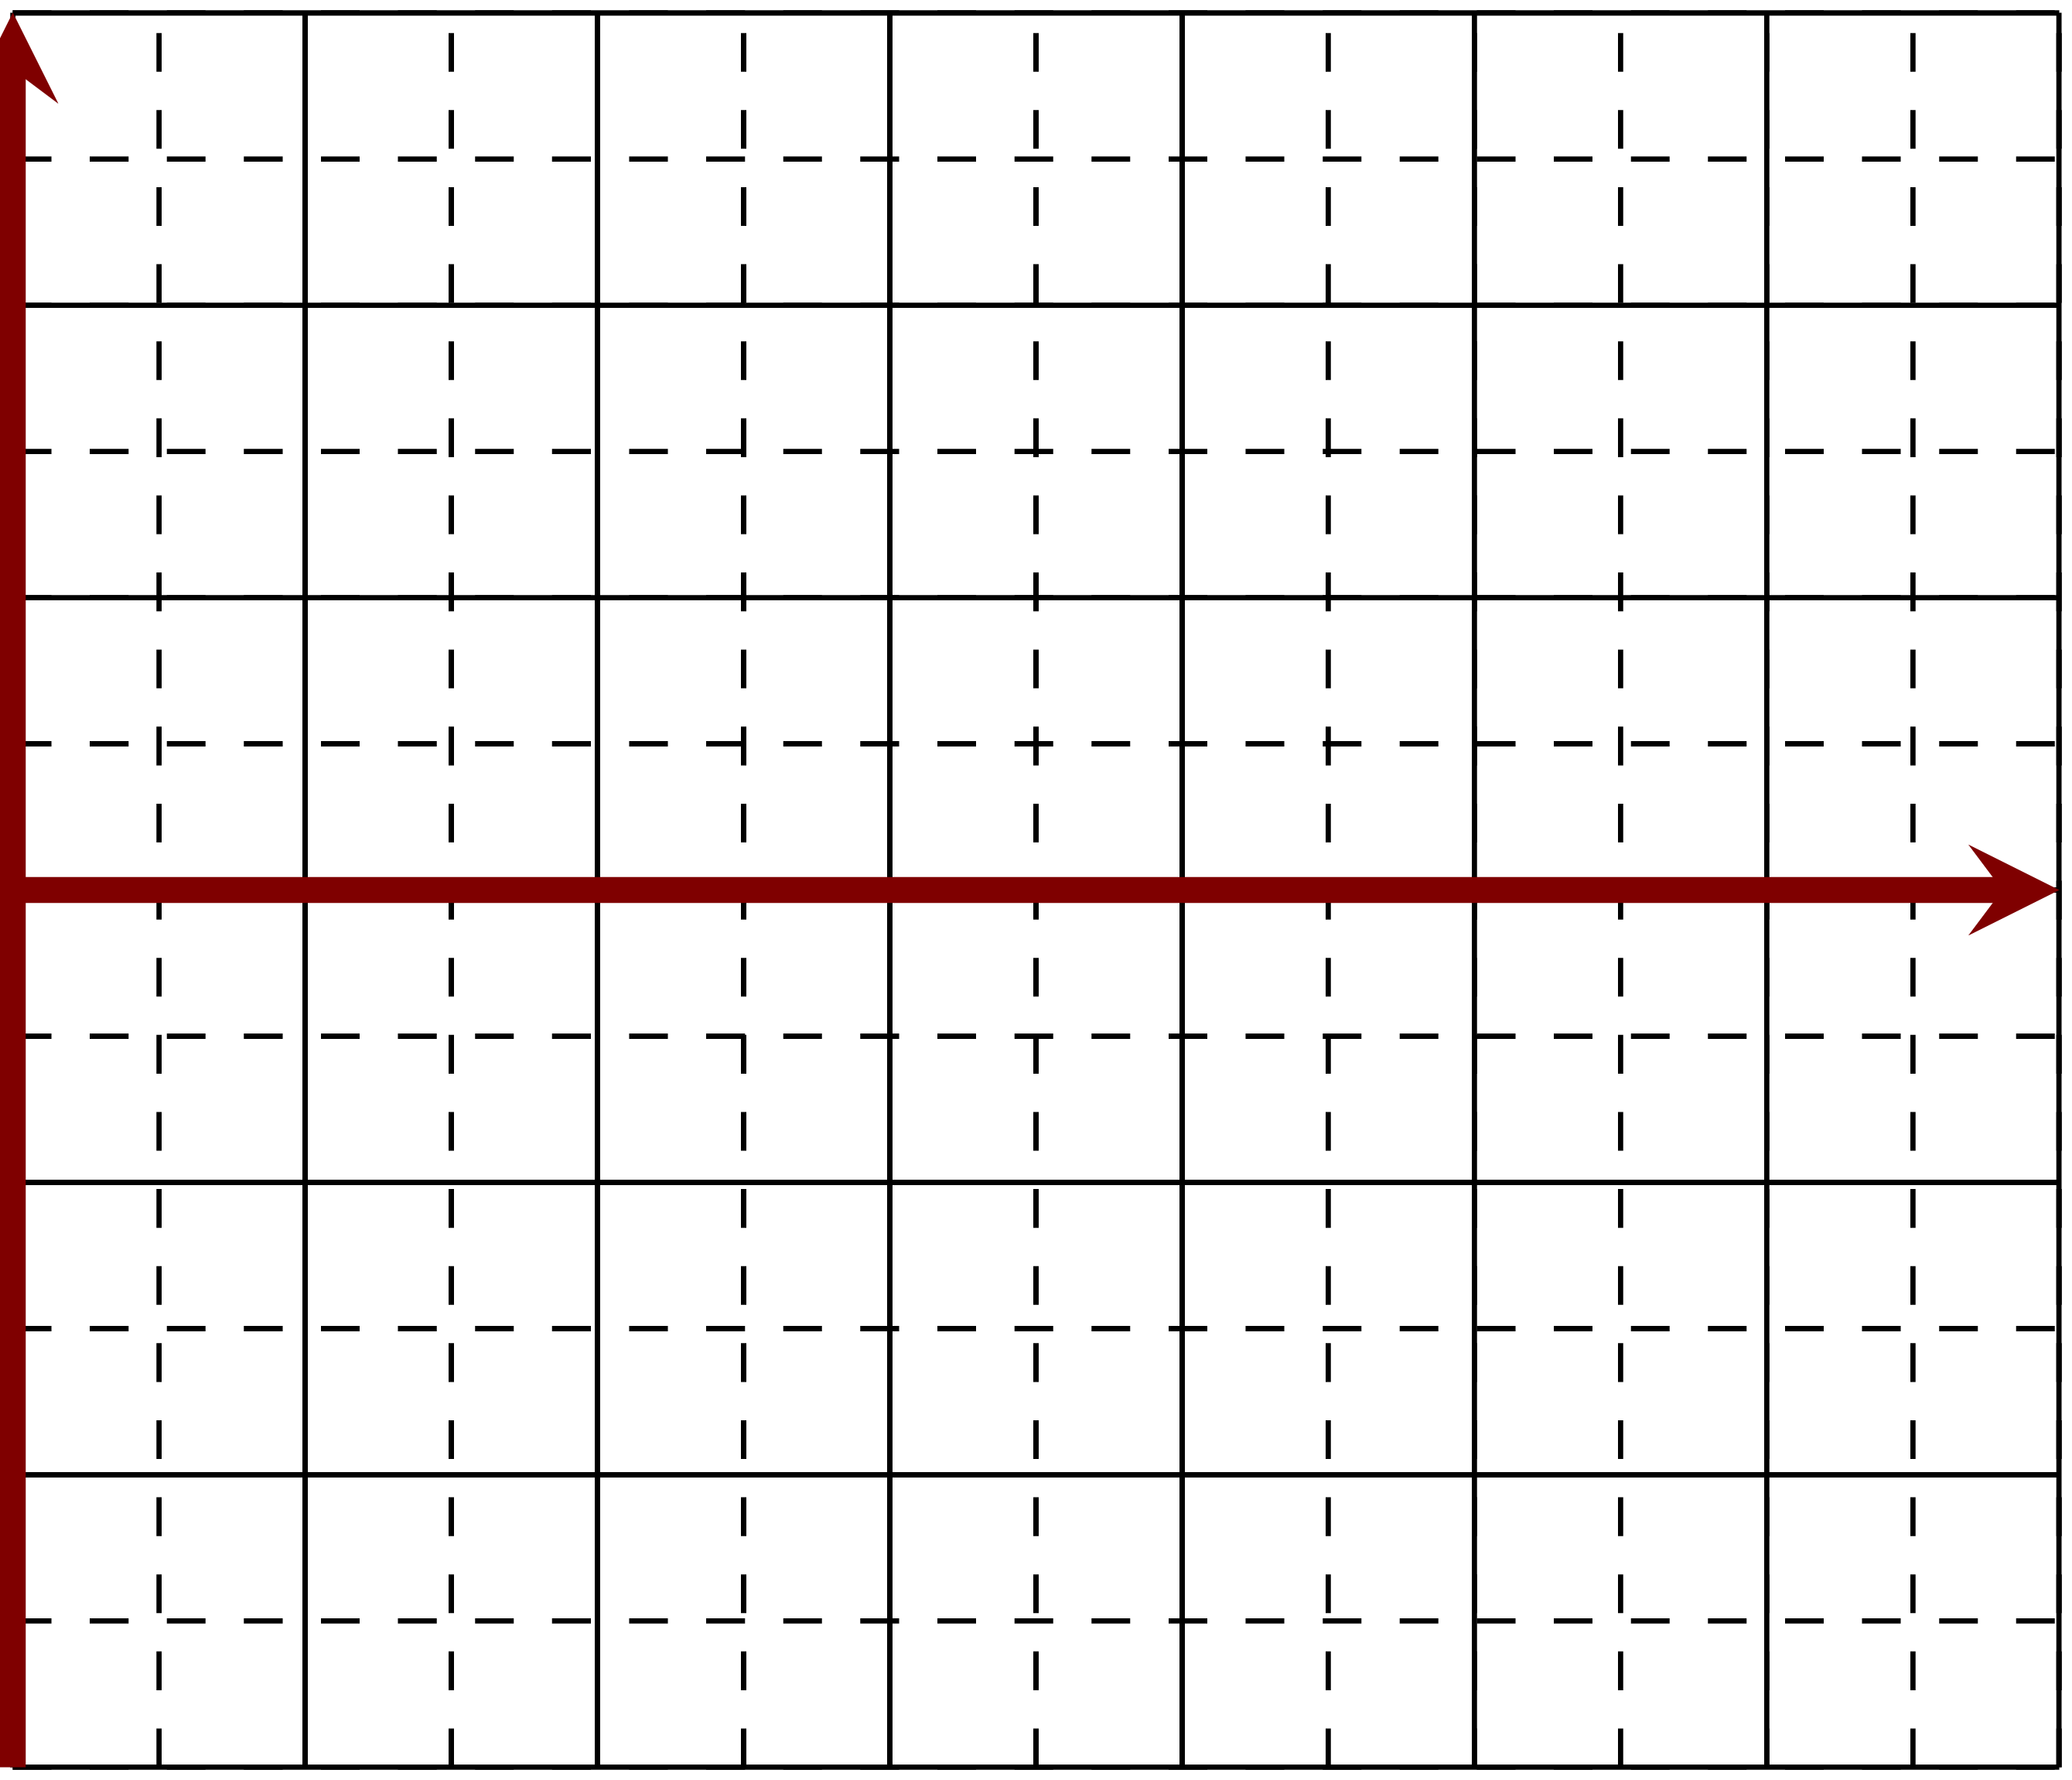
\includegraphics[scale=0.24,alt={Blank graph for adding values in a sequence},width=0.75\linewidth]{images/created/empty_seq_graph.png}
\end{sides}
\index{increasing}
\end{practiceprob}

% Alternating
\begin{practiceprob}
Consider \(c_n=(-2/3)^n\):
\begin{sides}
    \begin{itemize}
        \item \(c_0=\)
        \item \(c_1=\)
        \item \(c_2=\)
        \item \(c_3=\)
        \item \(c_4=\)
    \end{itemize}
    Description:
\tcblower
    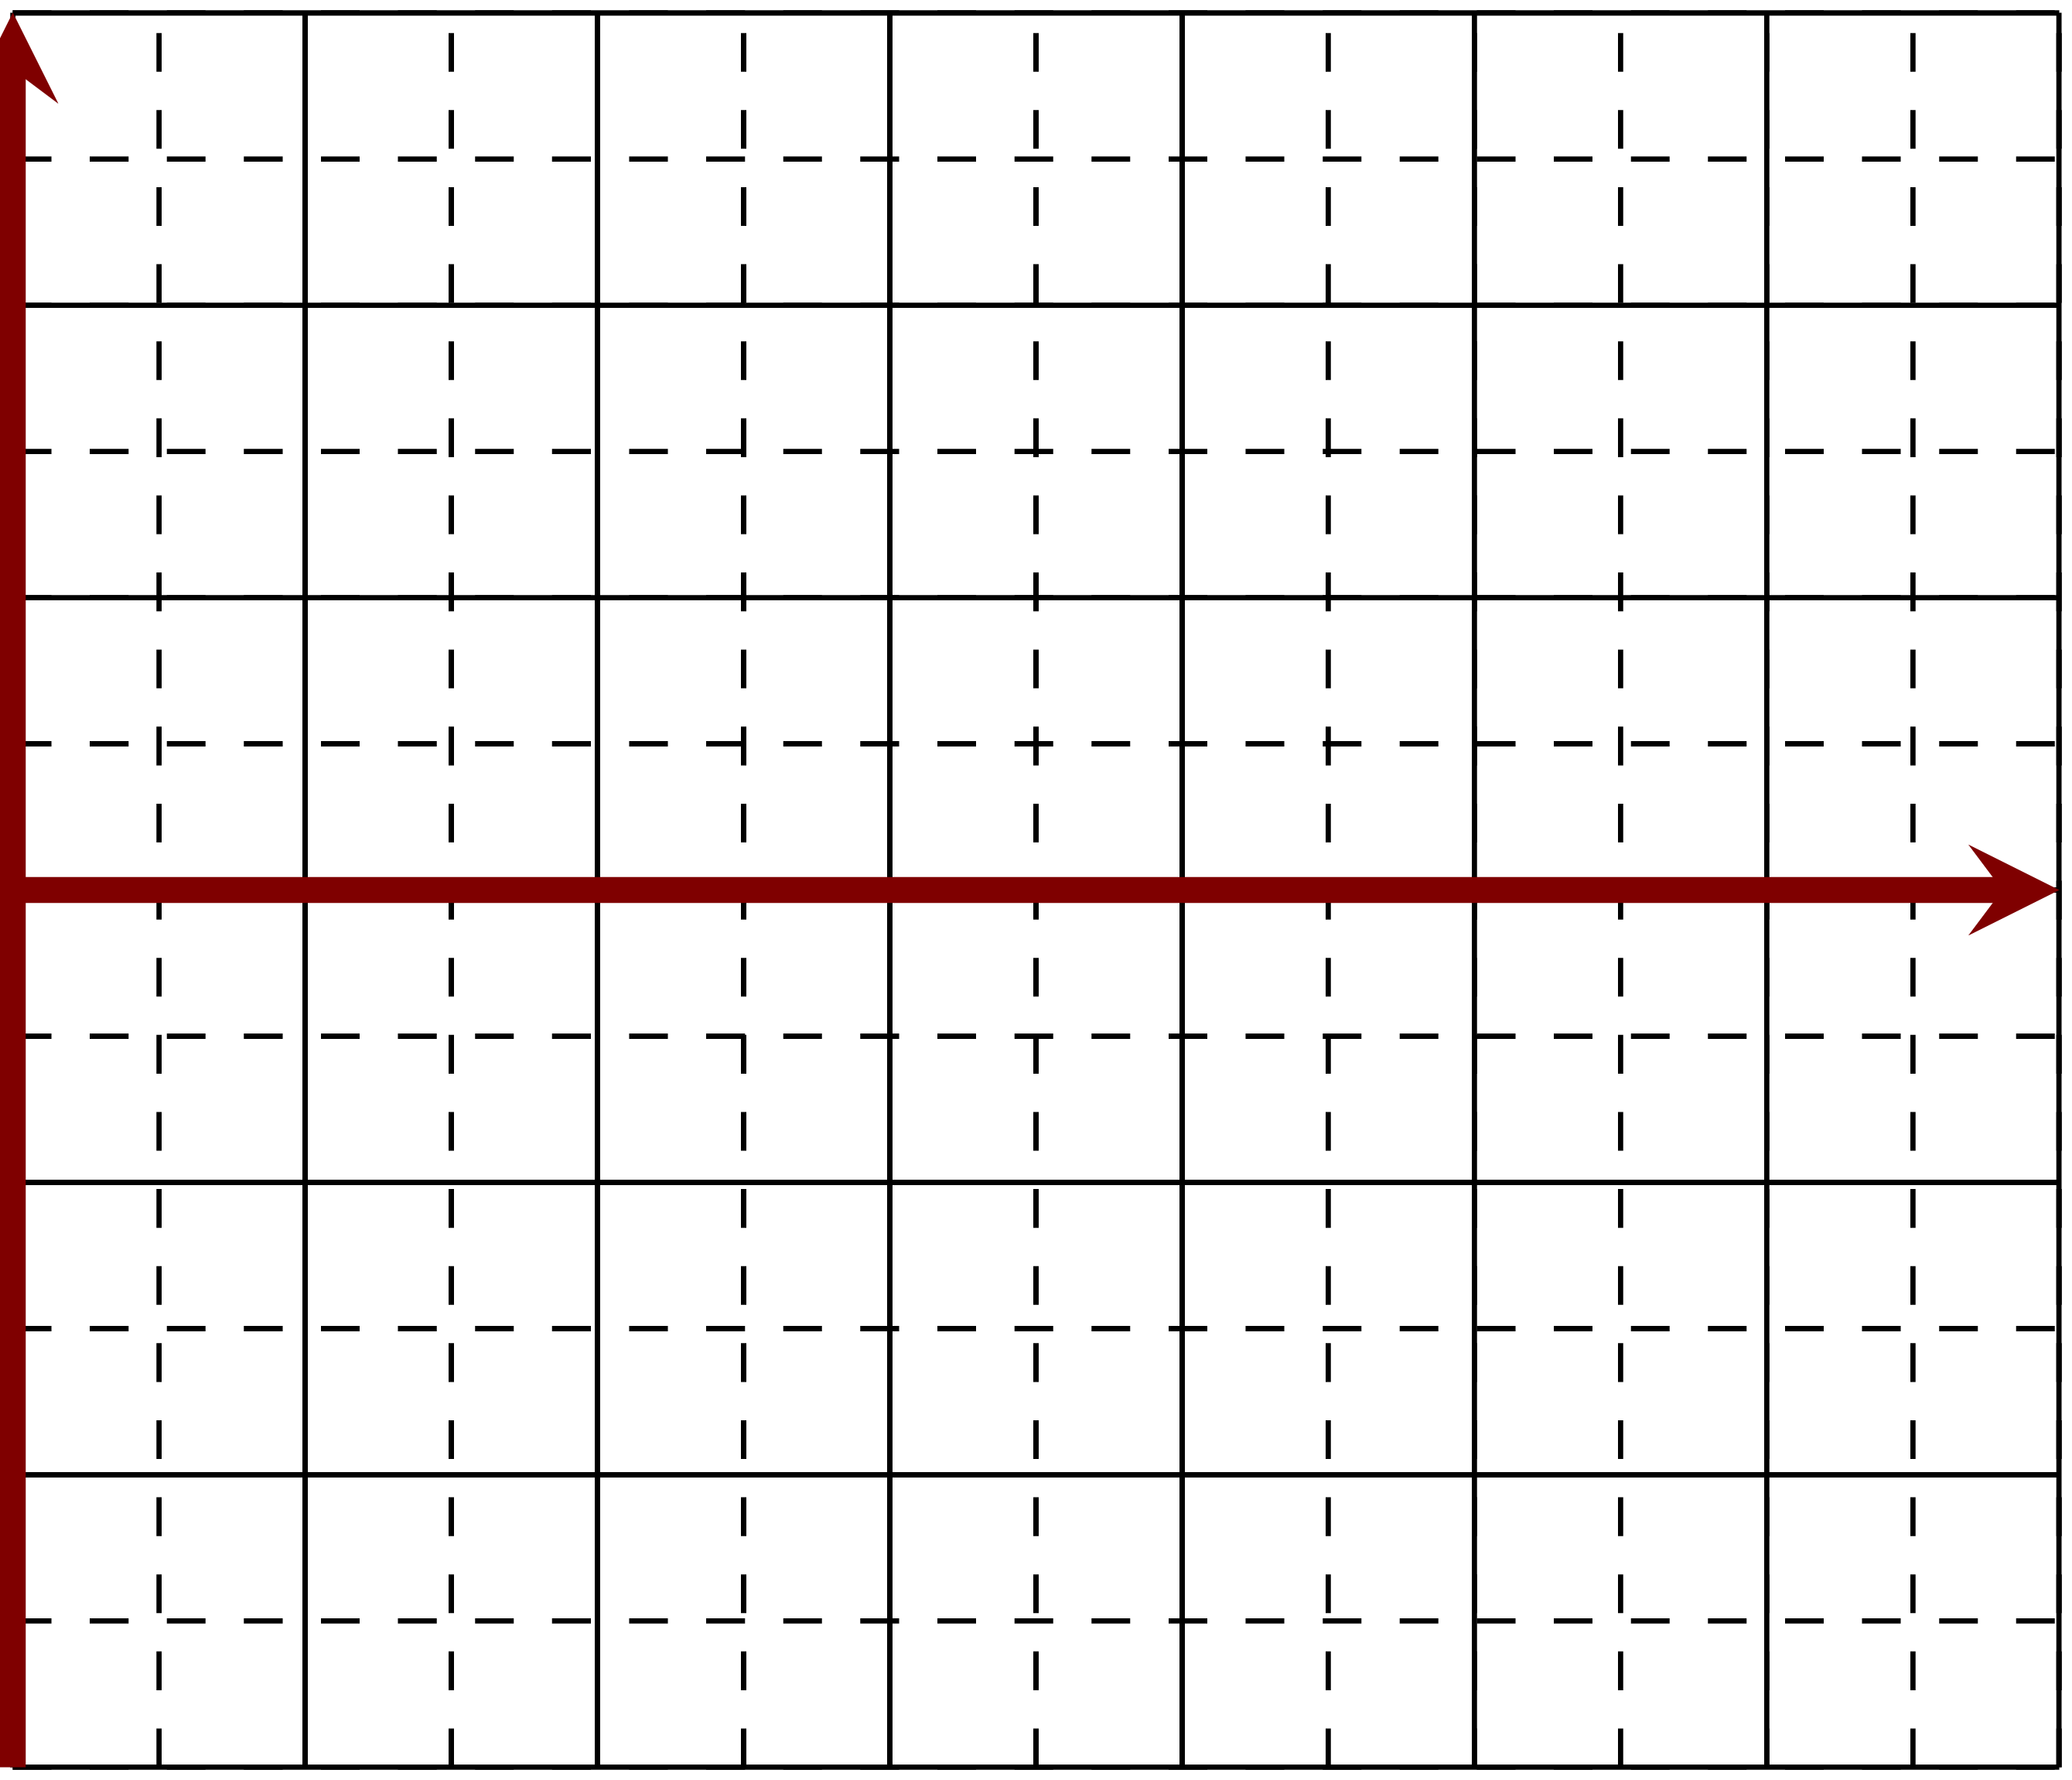
\includegraphics[scale=0.24,alt={Blank graph for adding values in a sequence},width=0.75\linewidth]{images/created/empty_seq_graph.png}
\end{sides}
\index{alternating}
\end{practiceprob}

% Increasing Bounded
\begin{practiceprob} Consider \(d_n=1-1/3^n\):
\begin{sides}
    \begin{itemize}
        \item \(d_0=\)
        \item \(d_1=\)
        \item \(d_2=\)
        \item \(d_3=\)
        \item \(d_4=\)
    \end{itemize}
    Description:
\tcblower
    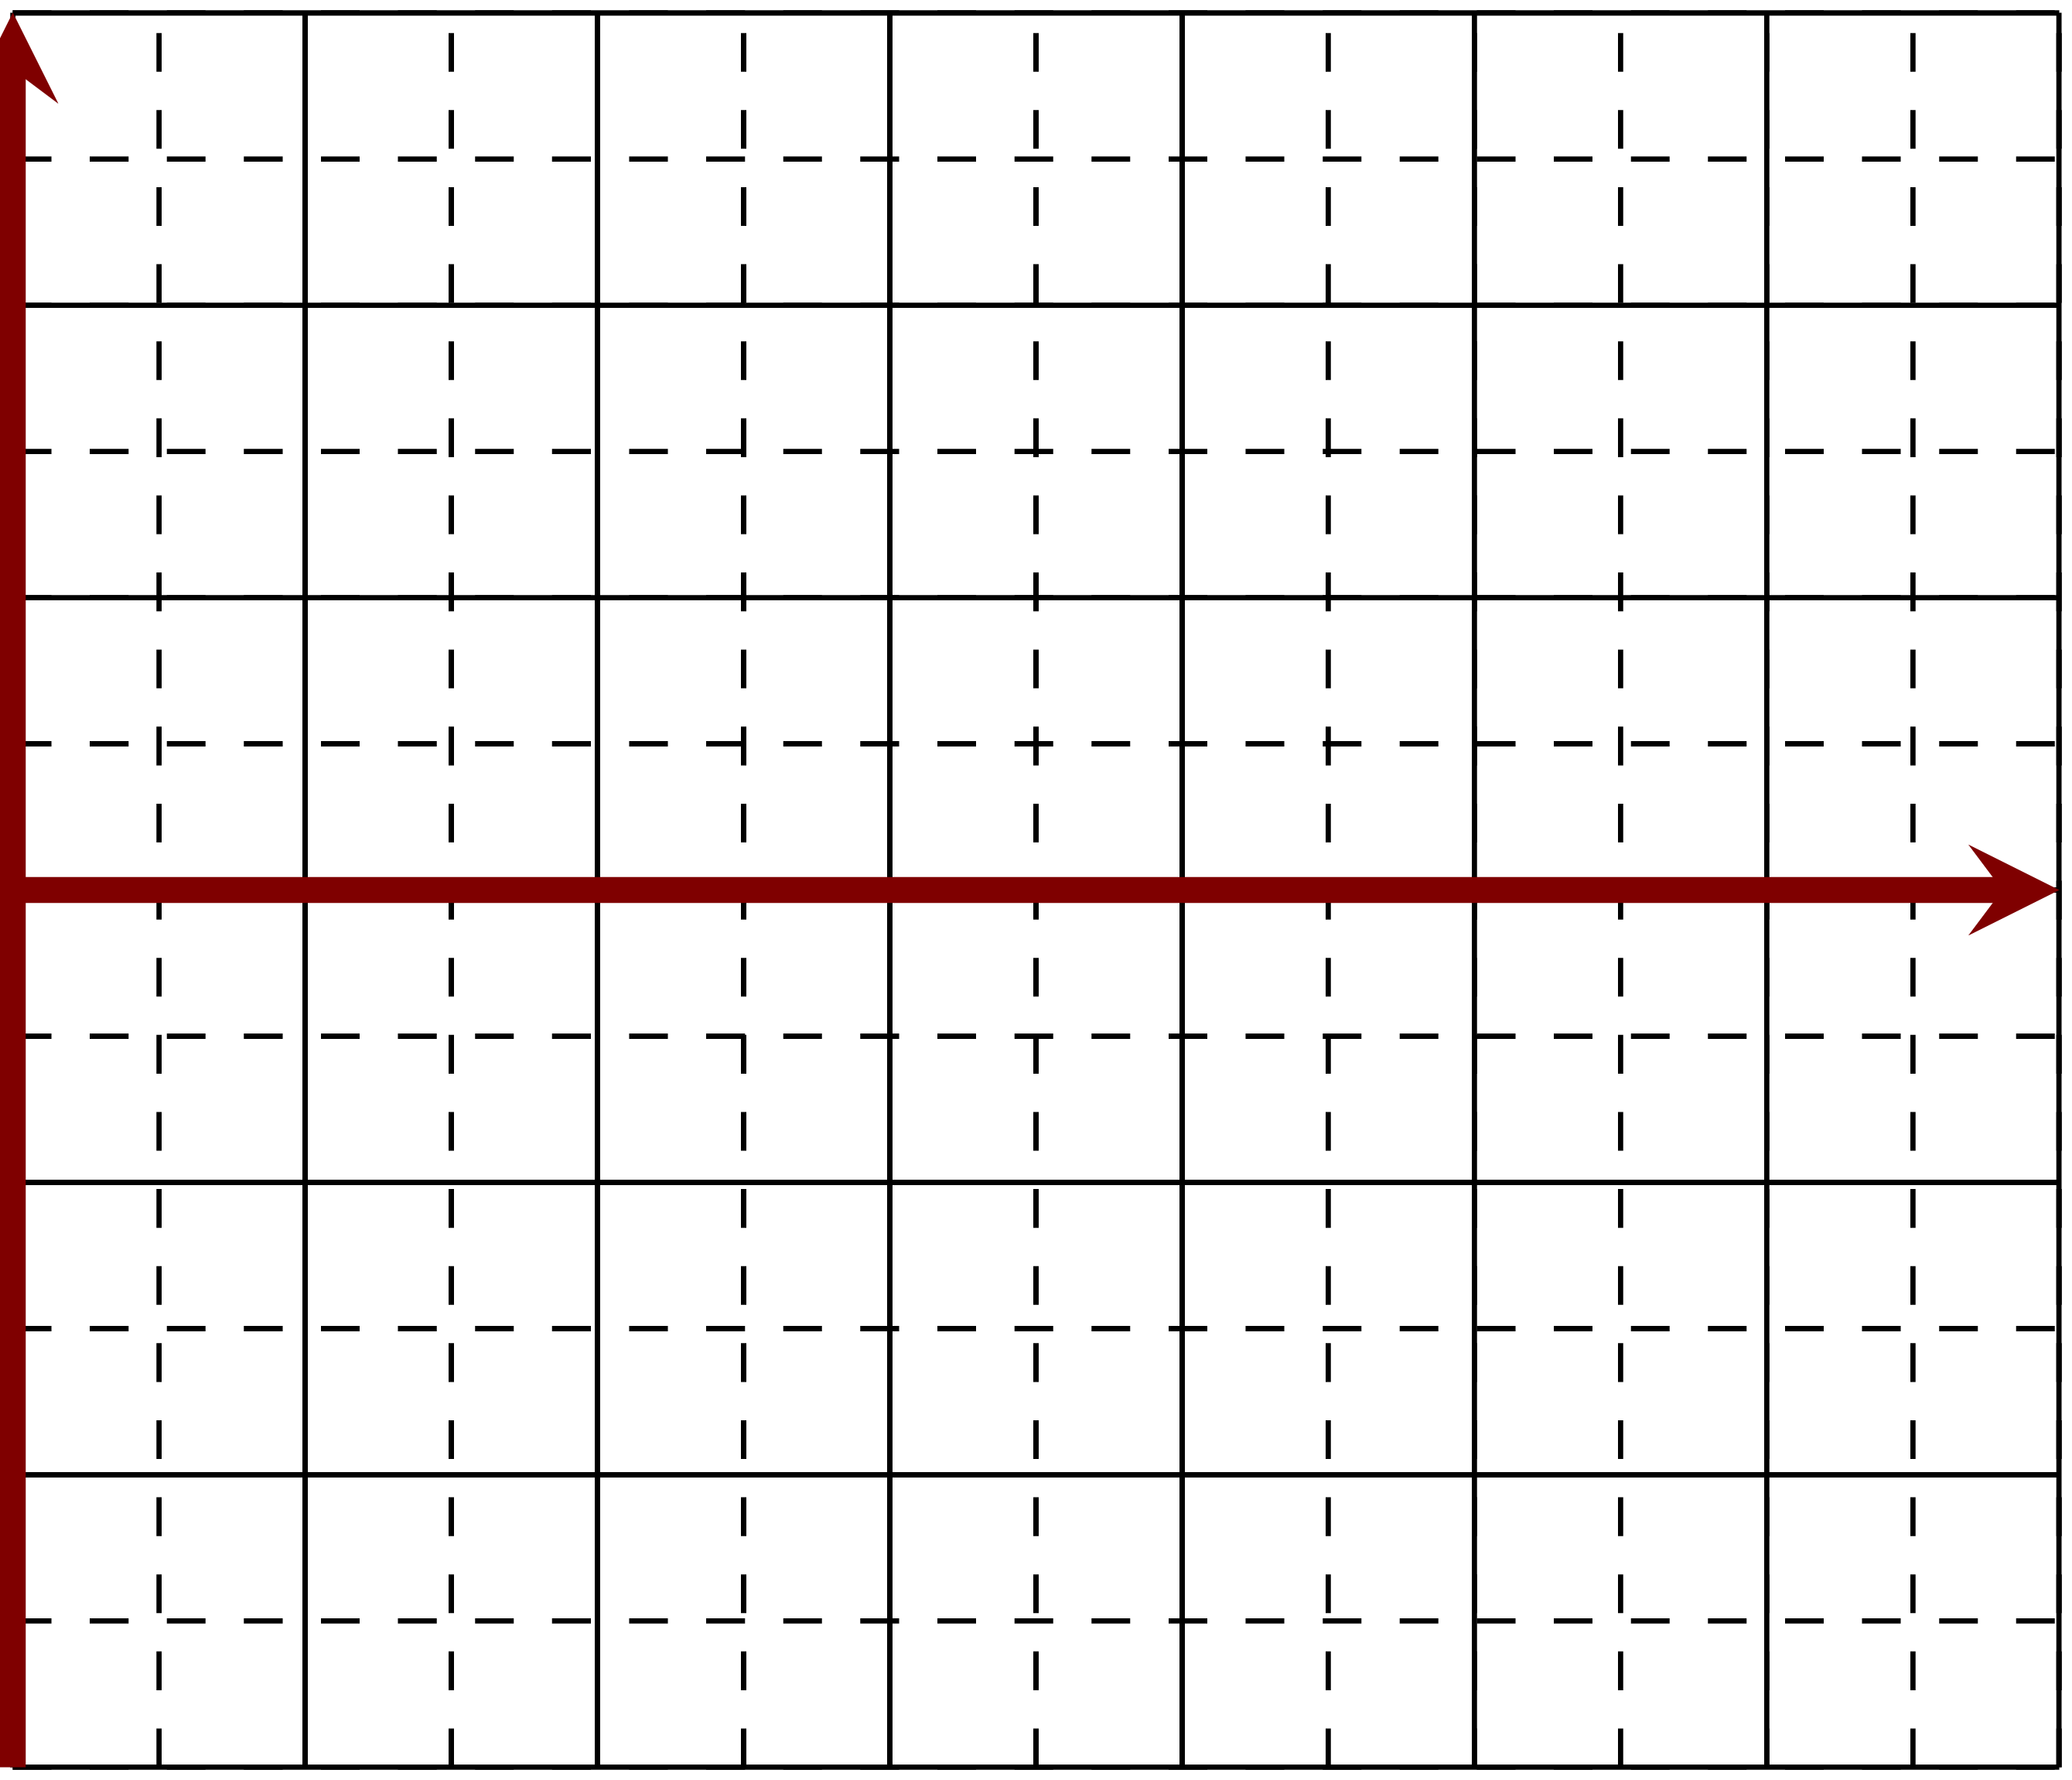
\includegraphics[scale=0.24,alt={Blank graph for adding values in a sequence},width=0.75\linewidth]{images/created/empty_seq_graph.png}
\end{sides}
\end{practiceprob}

% Alternating Bounded
\begin{practiceprob} Consider \(f_n=1+(-1/2)^n\):
\begin{sides}
    \begin{itemize}
        \item \(f_0=\)
        \item \(f_1=\)
        \item \(f_2=\)
        \item \(f_3=\)
        \item \(f_4=\)
    \end{itemize}
    Description:
\tcblower
    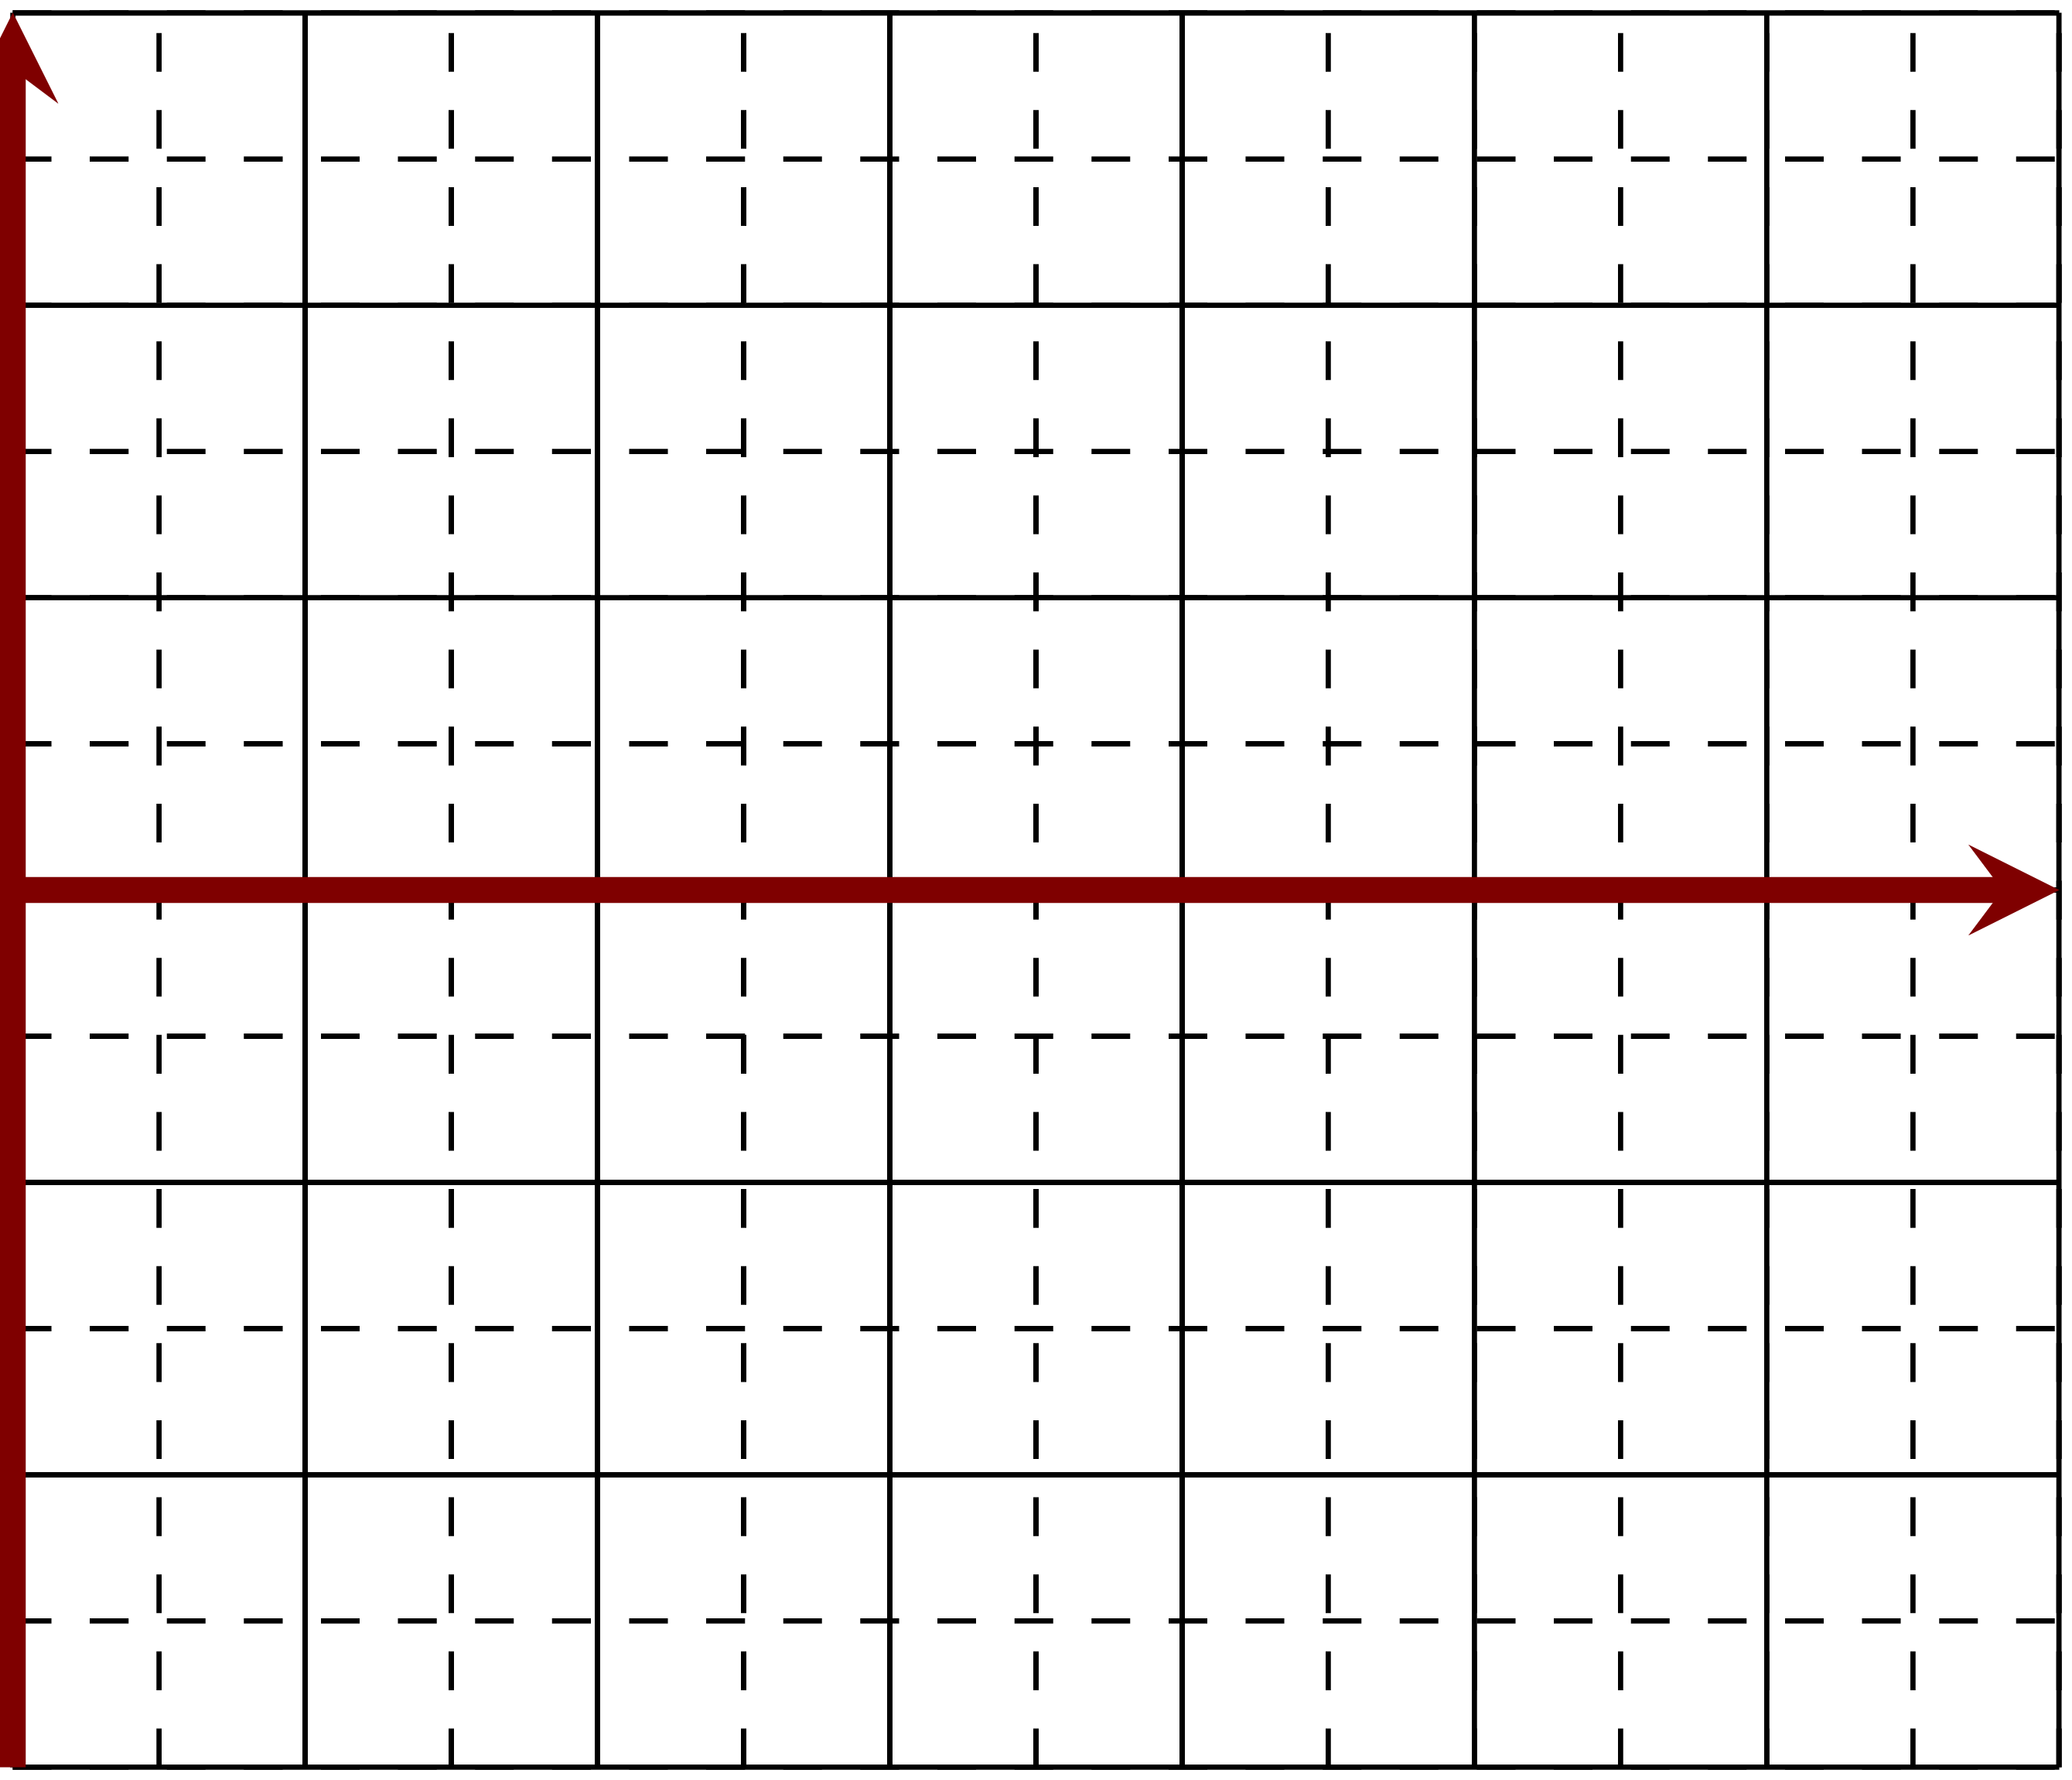
\includegraphics[scale=0.24,alt={Blank graph for adding values in a sequence},width=0.75\linewidth]{images/created/empty_seq_graph.png}
\end{sides}
\end{practiceprob}

% Aletrnating Convergent Sub Sequence
\begin{practiceprob} Consider \(h_n=(-1)^n+(-1/2)^n\):
\begin{sides}
    \begin{itemize}
        \item \(h_0=\)
        \item \(h_1=\)
        \item \(h_2=\)
        \item \(h_3=\)
        \item \(h_4=\)
    \end{itemize}
    Description:
\tcblower
    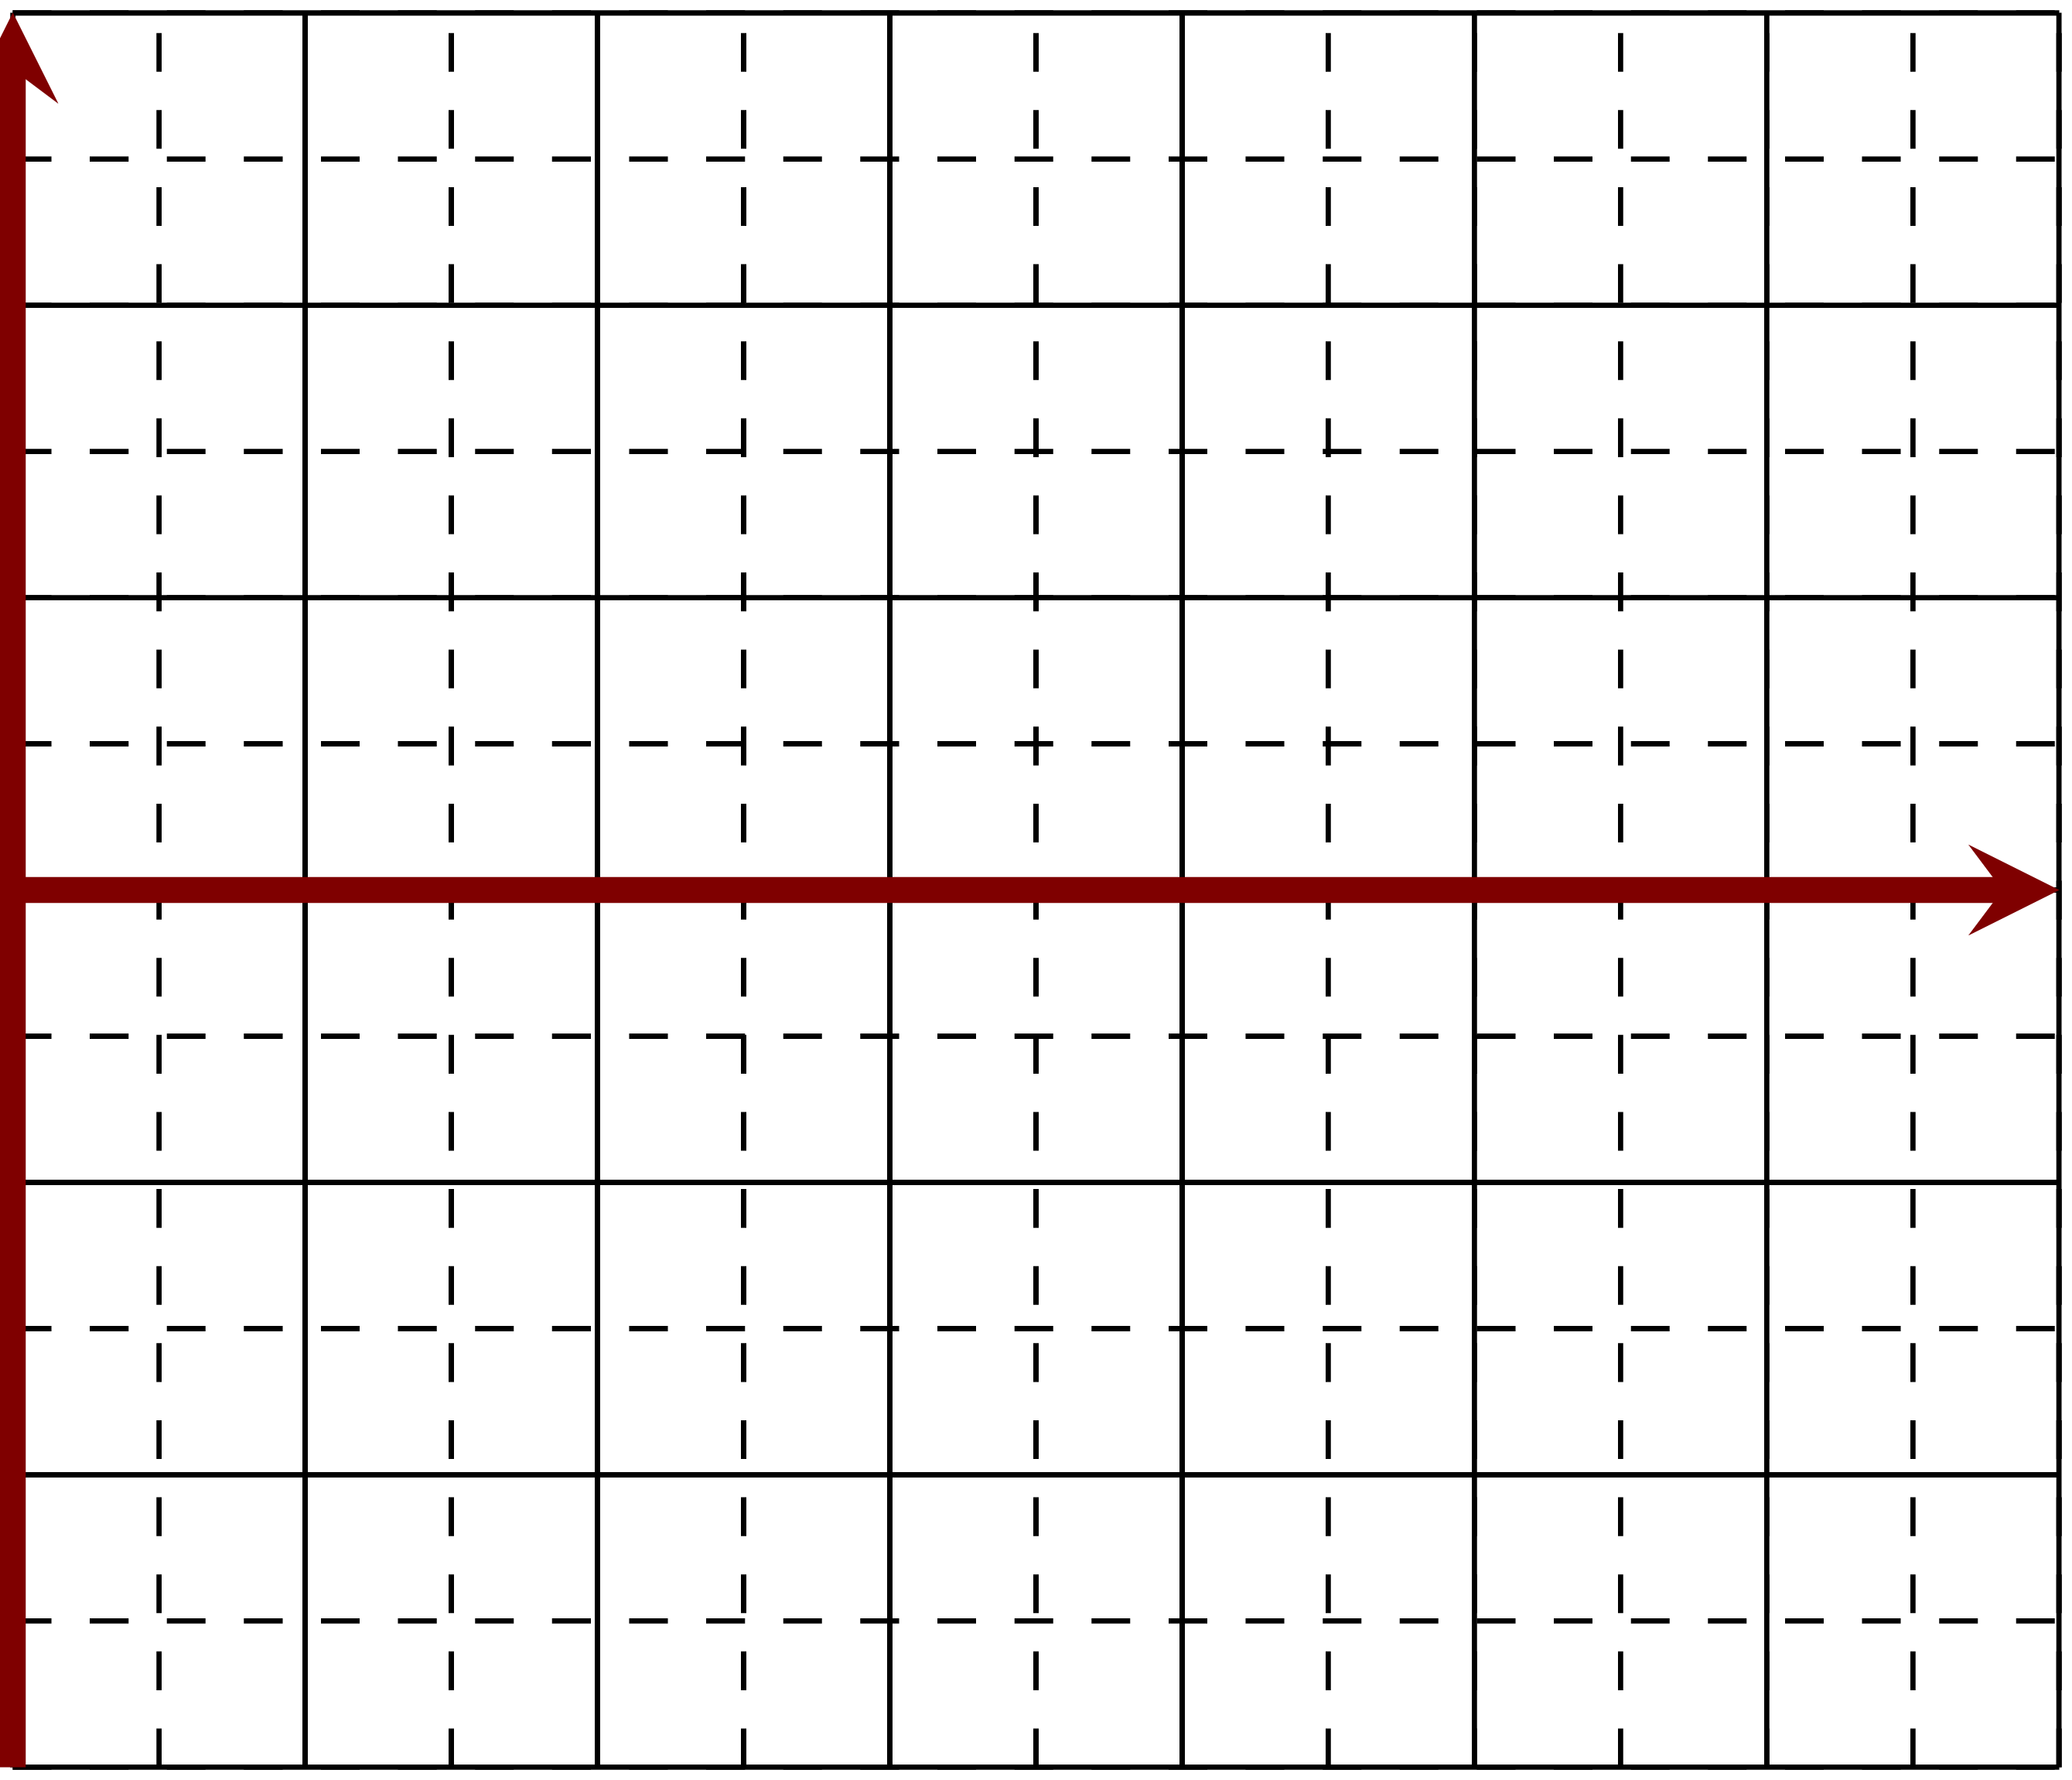
\includegraphics[scale=0.24,alt={Blank graph for adding values in a sequence},width=0.75\linewidth]{images/created/empty_seq_graph.png}
\end{sides}
\end{practiceprob}



% Aletrnating Convergent Sub Sequence
\begin{practiceprob} Consider \(j_n=(-1)^n-(-1/2)^n\):
\begin{sides}
    \begin{itemize}
        \item \(j_0=\)
        \item \(j_1=\)
        \item \(j_2=\)
        \item \(j_3=\)
        \item \(j_4=\)
        % \item \(j_5=\)
    \end{itemize}
    Description:
\tcblower
    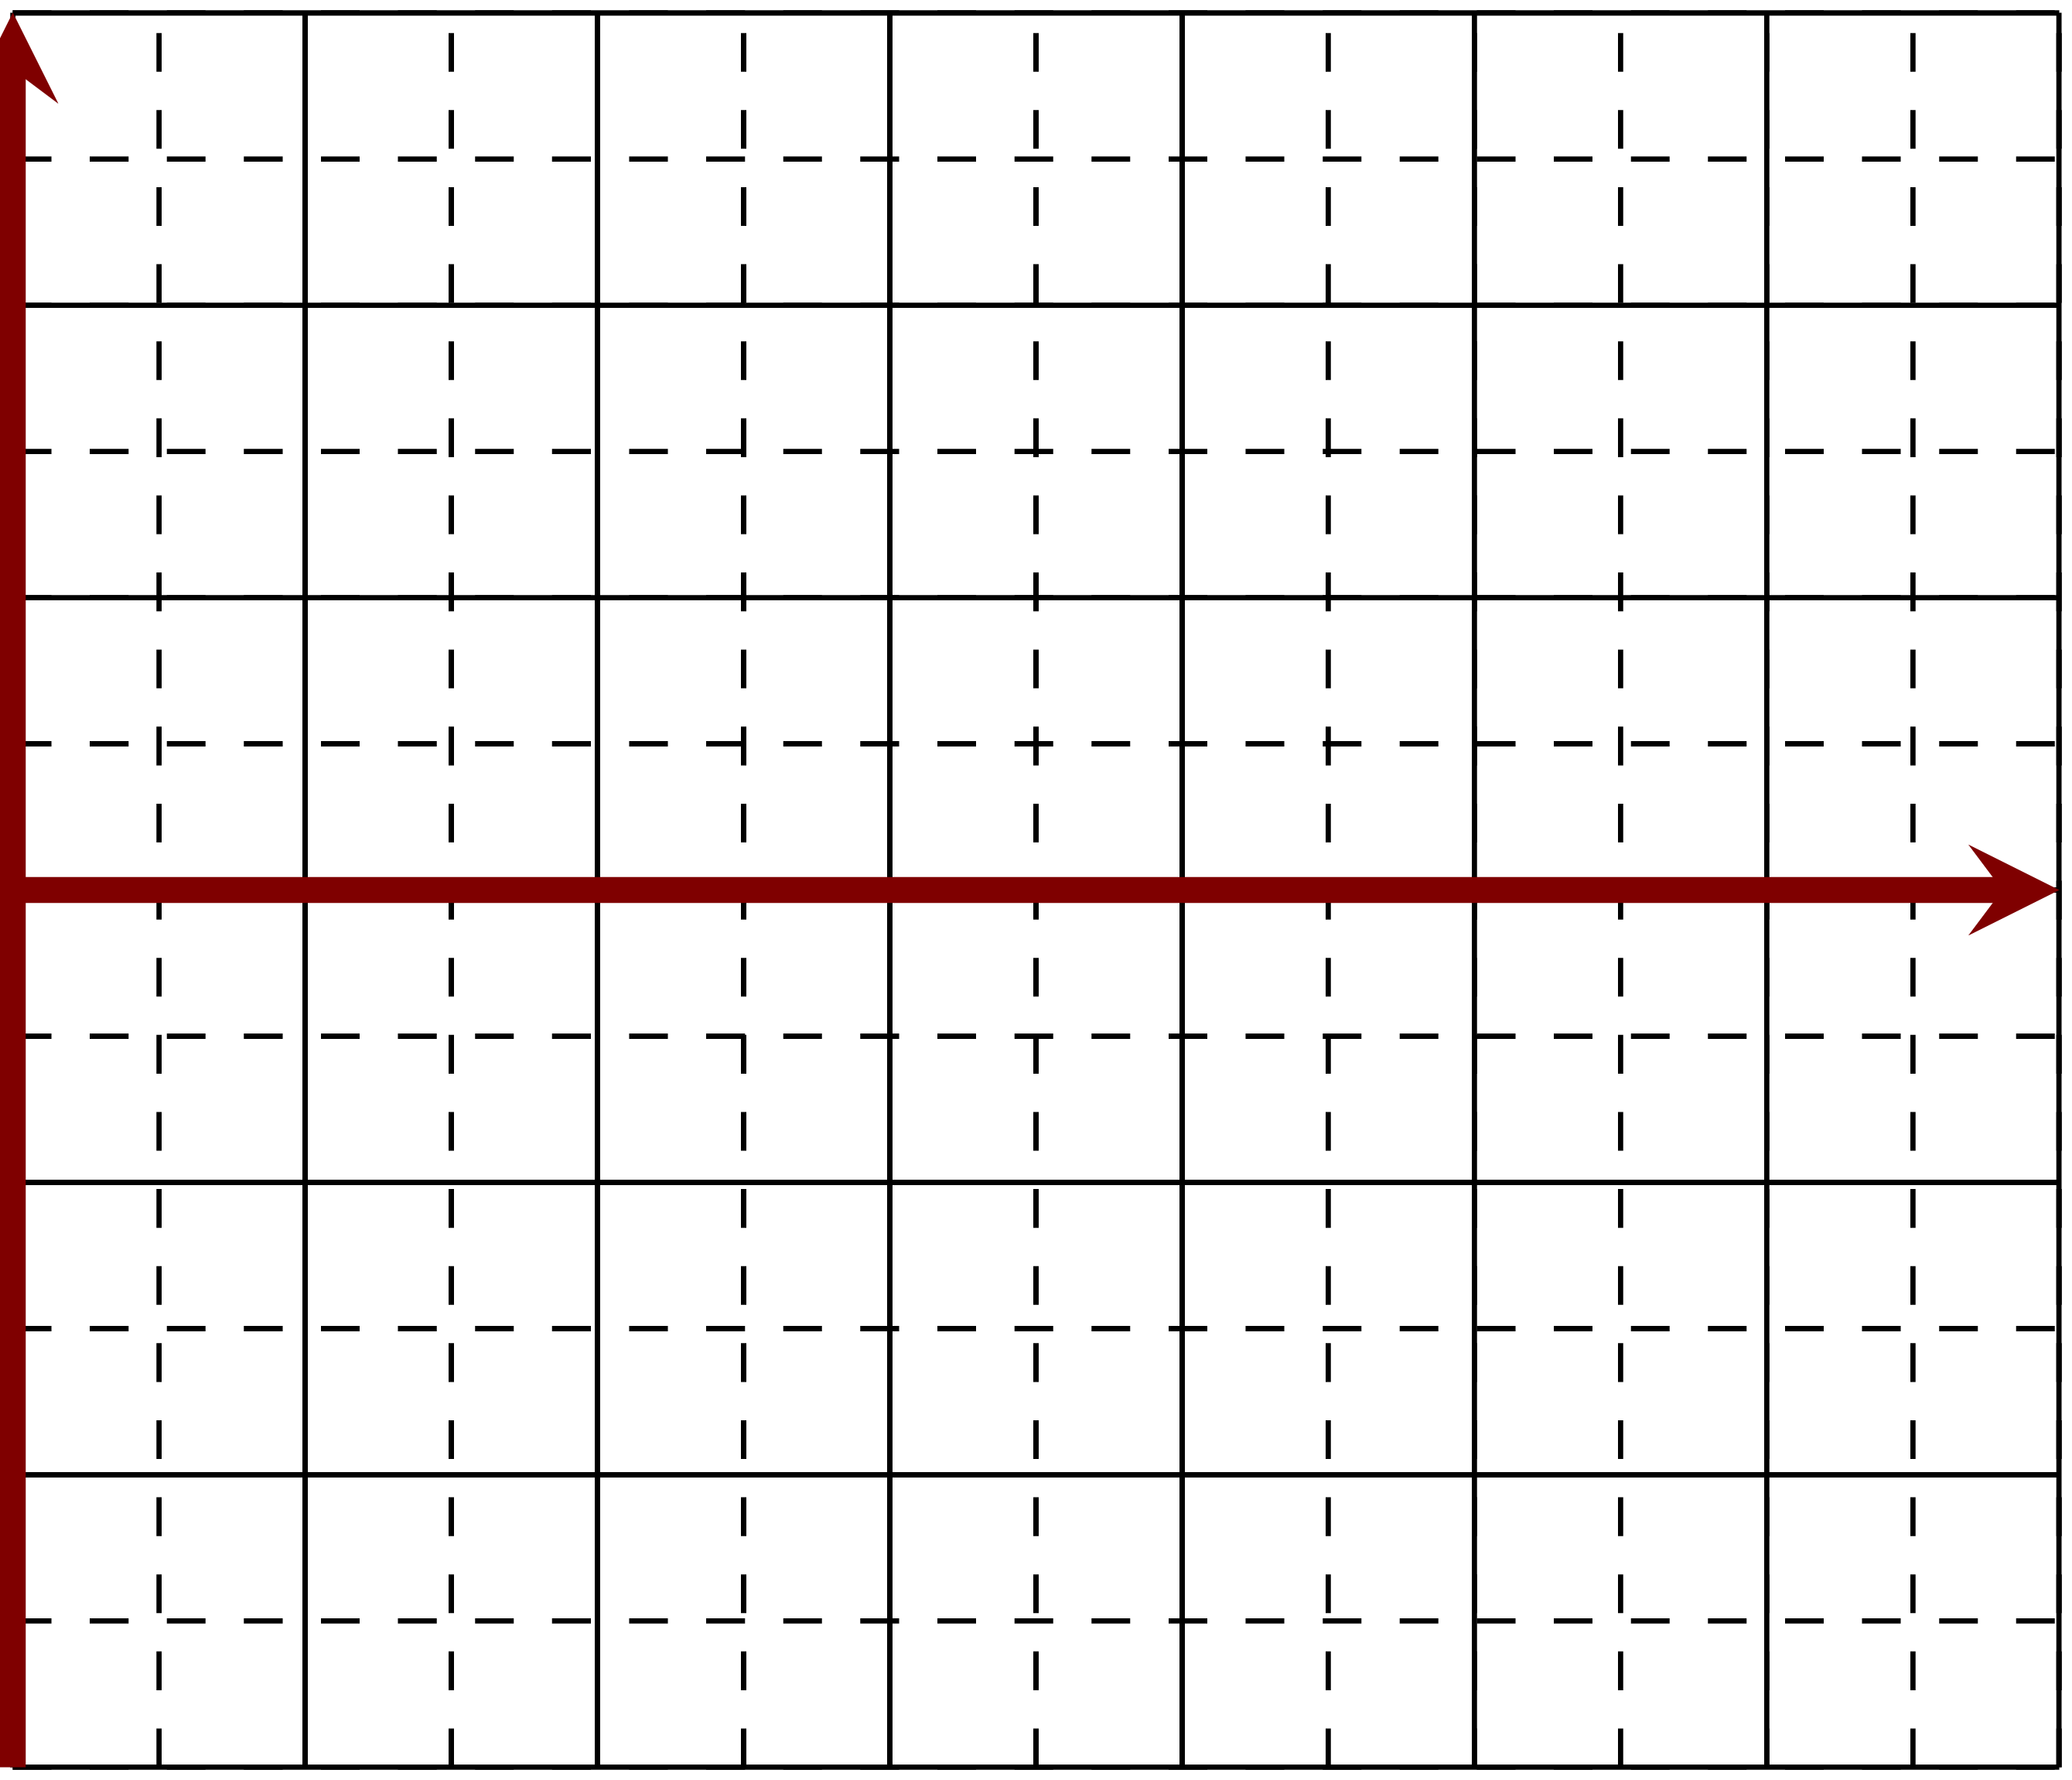
\includegraphics[scale=0.24,alt={Blank graph for adding values in a sequence},width=0.75\linewidth]{images/created/empty_seq_graph.png}
\end{sides}
\end{practiceprob}

\clearpage

\begin{thm}
    A bounded sequence has a \emph{convergent subsequence}. (The converse is not true.)
    \index{convergent}\index{subsequence}
\end{thm}

% Unbounded with a convergent subsequence
\begin{practiceprob} Consider \(k_n=0\) for even \(n\) and \(2^n\) for odd \(n\):
    \begin{itemize}
        \item \(k_0=\)
        \item \(k_1=\)
        \item \(k_2=\)
        \item \(k_3=\)
        \item \(k_4=\)
    \end{itemize}
    Description:
\end{practiceprob}


\begin{defn}[Recursive Sequence]
    A sequence is a \emph{recursive sequence}\index{recursive sequence} when the initial value is given explicitly, but subsequent values depend on previous values in the sequence.
\end{defn}

% Decreasing First Order Recursive 
\begin{practiceprob} Consider \(r_0=3\) and \(r_n=r_{n-1}/2\):
    \begin{itemize}
        \item \(r_0=\)
        \item \(r_1=\)
        \item \(r_2=\)
        \item \(r_3=\)
        \item \(r_4=\)
    \end{itemize}
    Description:
\end{practiceprob}

% \clearpage

% Increasing First Order Recursive 
\begin{practiceprob} Consider \(s_0=0\) and \(s_n=2s_{n-1}+1\):
    \begin{itemize}
        \item \(s_0=\)
        \item \(s_1=\)
        \item \(s_2=\)
        \item \(s_3=\)
        \item \(s_4=\)
    \end{itemize}
    Description:
\end{practiceprob}

% Increasing Second Order Recursive 

\begin{practiceprob}[Fibonacci Sequence] Consider \(F_0=1\), \(F_1=1\) and \(F_n=F_{n-1}+F_{n-2}\):
    \begin{itemize}
        \item \(F_0=\)
        \item \(F_1=\)
        \item \(F_2=\)
        \item \(F_3=\)
        \item \(F_4=\)
    \end{itemize}
    Description:
\end{practiceprob}

%%%% Find values in a recursive sequence starting with a high value.

\begin{practiceprob} Let's consider \[a_0=1\ \text{and}\ a_n=\frac{1}{3}a_{n-1},\] but this time we will work down from the value we want to the initial term (or \emph{base case}).\index{base case}
\begin{sides}
    Find \(a_5\):
    \begin{align*}
        a_5 &= \frac{1}{3} a_4 && a_n=\frac{1}{3}a_{n-1}\\
            &= \phantom{\rule{100pt}{30pt}} && a_n=\frac{1}{3}a_{n-1}\\
            &= \phantom{\rule{60pt}{30pt}} && a_n=\frac{1}{3}a_{n-1}\\
            &= \phantom{\rule{60pt}{30pt}} && a_n=\frac{1}{3}a_{n-1}\\
            &= \phantom{\rule{60pt}{30pt}} && a_n=\frac{1}{3}a_{n-1}\\
            &= \phantom{\rule{60pt}{30pt}} && a_0=1\\
    \end{align*}
\tcblower
    Find \(a_{10}\):
    \begin{align*}
        a_{10} &= \frac{1}{3} a_{9} && a_n=\frac{1}{3}a_{n-1}\\
            &= \phantom{\rule{100pt}{30pt}} && a_n=\frac{1}{3}a_{n-1}\\
            &= \phantom{\rule{100pt}{30pt}} && a_n=\frac{1}{3}a_{n-1}\\
            &= \phantom{\rule{100pt}{30pt}} && a_n=\frac{1}{3}a_{n-1}\\
            &= \phantom{\rule{100pt}{30pt}} && a_n=\frac{1}{3}a_{n-1}\\
            &= \phantom{\rule{100pt}{30pt}} && a_5=\\
    \end{align*}
\end{sides}
\end{practiceprob}

\begin{practiceprob} Using \[b_0=1\ \&\ b_1=2\ \text{and}\ b_n=b_{n-1}+2b_{n-2},\]
    find \(b_5\):
    \begin{align*}
        b_5 &= 2 b_4+2b_3 && b_n=b_{n-1}+2b_{n-2}\\
            &= \phantom{\rule{150pt}{40pt}} && b_n=b_{n-1}+2b_{n-2}\\
            &= \phantom{\rule{100pt}{40pt}} && b_n=b_{n-1}+2b_{n-2}\\
            &= \phantom{\rule{100pt}{40pt}} && b_n=b_{n-1}+2b_{n-2}\ \&\ b_1=2\\
            &= \phantom{\rule{60pt}{40pt}} && b_0=1\ \&\ b_1=2\\
    \end{align*}
\end{practiceprob}

\clearpage

\subsection{Finding Sequence Formulas}

% Arithmetic Example
\begin{practiceprob}
    Given the following values determine a formula for the sequence:
    \[a_0=1, a_1=5, a_2=9, a_3=13, a_4=17, \ldots\]
    \vspace{4\baselineskip}
\end{practiceprob}

% Geometric Example
\begin{practiceprob}
    Given the following values determine a formula for the sequence:
    \[b_0=3, b_1=12, b_2=48, b_3=192, a_4=768, \ldots\]
    \vspace{4\baselineskip}
\end{practiceprob}

% General Example
\begin{practiceprob}
    Given the following values determine a formula for the sequence:
    \[c_0=\frac{-1}{2}, c_1=\frac{1}{6}, c_2=\frac{-1}{12}, c_3=\frac{1}{20}, c_4=\frac{-1}{30}, \ldots\]
    \vspace{4\baselineskip}
\end{practiceprob}

% First Order Recursive Example
\begin{practiceprob}
    Given the following values determine a formula for the sequence:
    \[d_0=1, d_1=5, d_2=13, d_3=29, d_4=61, \ldots\]
    \vspace{4\baselineskip}
\end{practiceprob}

\clearpage

% Second Order Recursive Example
\begin{practiceprob}
    Given the following values determine a formula for the sequence:
    \[e_0=2, e_1=3, e_2=7, e_3=13, e_4=27, \ldots\]
    \vspace{4\baselineskip}
\end{practiceprob}

%   - $a_n = 3^n - 2$ or $a_n=a_{n-1}+6\cdot 3^{n-2}$
\begin{practiceprob}
    Given the following values determine a formula for the sequence:
    \[f_1=1, f_2=7, f_3=25, f_4=79, f_5=241, \ldots\]
    \vspace{4\baselineskip}
\end{practiceprob}

% - Repeat n n times: $a_n = floor(\sqrt{2n} + 1/2)$
% - Add note about the On-Line Encyclopedia of Integer Sequences (OEIS) (https://oeis.org/) as well as citation to the Encyclopedia
\begin{practiceprob}
    Given the following values try to describe the sequence, then use the \emph{On-Line Encyclopedia of Integer Sequences} (OEIS) (\url{https://oeis.org/}) to get the formula.
    \[g_1=1, g_2=22, g_3=333, g_4=4444, g_5=55555, \ldots\]
    \vspace{4\baselineskip}
\end{practiceprob}



